%% Dokumentenklasse (Koma Script) -----------------------------------------
\documentclass[%
   11pt,              % Schriftgroesse
   ngerman,           % wird an andere Pakete weitergereicht
   a4paper,           % Seitengroesse
   DIV11,             % Textbereichsgroesse (siehe Koma Skript Dokumentation !)
]{scrartcl}%     Klassen: scrartcl, scrreprt, scrbook
% -------------------------------------------------------------------------

\usepackage[utf8]{inputenc} % Font Encoding, benoetigt fuer Umlaute
\usepackage[ngerman]{babel}   % Spracheinstellung

\usepackage[T1]{fontenc} % T1 Schrift Encoding
\usepackage{textcomp}    % Zusatzliche Symbole (Text Companion font extension)
\usepackage{lmodern}     % Latin Modern Schrift
\usepackage{listings}
\usepackage{framed}
\usepackage{amssymb}
\usepackage{amsmath}
\usepackage{framed}
\usepackage{listings}
%für die Konfusionsmatrizen
\usepackage{csvsimple}
\usepackage{lscape}


\usepackage[left=2cm,right=3cm,top=2cm,bottom=2cm,includeheadfoot]{geometry}
%Kopf- und Fußzeile
\usepackage{fancyhdr}
%Grafiken einbetten
\usepackage{graphicx}

\pagestyle{fancy}
\fancyhf{}
%Übungsteilnehmer
\fancyhead[L]{Matthias Hansen, 331600~~Lukas Huwald, 322890\\}
%Kopfzeile mittig
\fancyhead[R]{NLP Exercise03}
%Linie oben
\renewcommand{\headrulewidth}{0.5pt}

\setlength{\parskip}{1ex}

%Fußzeile links bzw. innen
\fancyfoot[L]{}
%Fußzeile rechts bzw. außen
\fancyfoot[R]{\thepage}
%Linie unten
\renewcommand{\footrulewidth}{0.5pt}
%% Dokument Beginn %%%%%%%%%%%%%%%%%%%%%%%%%%%%%%%%%%%%%%%%%%%%%%%%%%%%%%%%
\begin{document}
\section*{Task 1}
\subsection*{a.)}

See code and especially the file \texttt{README.txt}.

\subsection*{b.)}

In addition to classification accuracy, we have also plotted the percentage
of documents that the classifier rejected. Our classifier rejects a document
if p(c|document) is 0 for all classes c. In our program, this corresponds to the log-likelihood coming out as \texttt{-inf}.

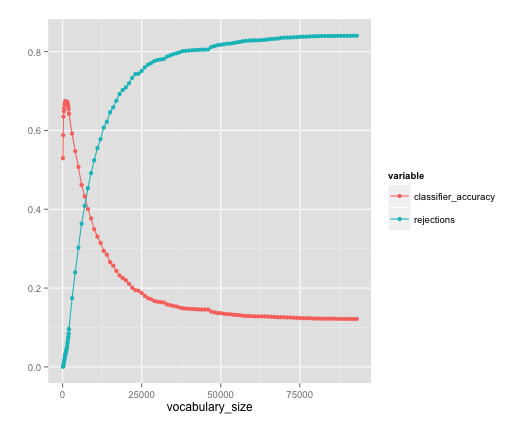
\includegraphics[width=\textwidth]{exercise03.1/accuracy_naive.png}

As we can see, the error rate shows this behavior because too many Documents are rejected due to p(c|document) being zero. This is the case because of p(document|c) being 0 in the Bayes decision rule. p(document|c) is just the product of the relative frequencies of the words of the document in the training data, however. So, to conclude, the problem is that as soon as one word that was not encountered in the training data is encountered in a test document, the test document will get rejected immediately. This occurs most frequently when the dictionary is large, because in a small dictionary, these rare words just get replaced by \texttt{<UNK>}, which is then a very frequent word.

\subsection*{c.)}

To solve this problem, we propose to use a simple smoothing method.
Originally, the class conditional probabilities of words are defined as follows:

$p(w|c) = \frac{N_{w,c}}{N_c}$

However, the problem was that $N_{w,c}$ was zero frequently. To solve this, we replace the cases in which it was zero by one.

$p(w|c) = \begin{cases} 
    p(w|c) = \frac{1}{N_c} & \text{if } N_{w,c} = 0\\
    p(w|c) = \frac{N_{w,c}}{N_c} & \text{otherwise}\\
\end{cases}$

However, in this solution, the probabilites do not add up to 1, which is a problem. To fix this, we introduce a ``count count'' $N_0 := |\{w|N_{w,c} = 0\}|$. And write the probability as follows.

$p(w|c) = \begin{cases} 
    p(w|c) = \frac{1}{N_c + N_0} & \text{if } N_{w,c} = 0\\
    p(w|c) = \frac{N_{w,c}}{N_c + N_0} & \text{otherwise}\\
\end{cases}$

Now that we have solved this problem, the accuracy is much better, especially for bigger vocabularies:

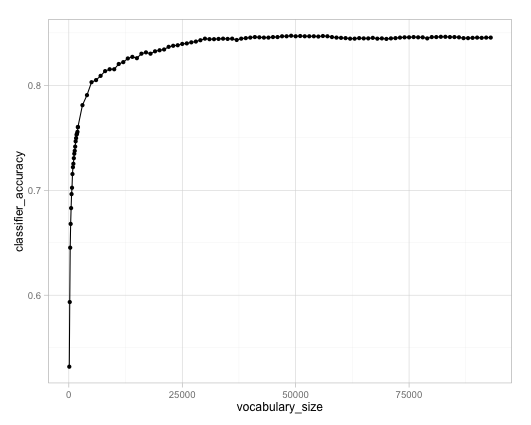
\includegraphics[width=\textwidth]{exercise03.1/accuracy_smoothed.png}


\makeatletter
\csvset{
autotabularcenter/.style={
    file=#1,
    after head=\csv@pretable\begin{tabular}{|*{\csv@columncount}{p{1.5cm}|}}\csv@tablehead,
    table head=\hline\csvlinetotablerow\\\hline,
    late after line=\\\hline,
    table foot=\\\hline,
    late after last line=\csv@tablefoot\end{tabular}\csv@posttable,
    command=\csvlinetotablerow},
}
\makeatother
\newcommand{\csvautotabularcenter}[2][]{\csvloop{autotabularcenter={#2},#1}}

\begin{landscape}
\subsection*{d.)}

Confusion matrix for smoothed probabilities:

\scalebox{0.5} {
    \csvautotabularcenter{exercise03.1/confusion_matrix_smoothed.csv}
}
\end{landscape}

\begin{landscape}

Confusion matrix for unsmoothed probabilities:

\scalebox{0.5} {
    \csvautotabularcenter{exercise03.1/confusion_matrix.csv}
}
\end{landscape}



\end{document}
